\chapter{Мощность множества}

%pwr: prefix
Дается более строгое определение мощности. Для углубленного изучения рекомендуются \cite{bib:sudoplatov:discrmath,bib:shaporev:discretemath}.


\section{Основные теоремы и определения}

Множества $A$ и $B$ называются \emph{эквивалентными} (обозначается $A\sim B$), если существует биекция $f:A\leftrightarrow B$.

\begin{enumerate}
	\item $A\sim A$ (так как существует $I_A:A\leftrightarrow A$);
	\item Если $A\sim B$, то $B\sim A$ (так как существует $f:A\leftrightarrow B$, то существует и $f^{-1}:B\leftrightarrow A$);
	\item Если $A\sim B$ и $B\sim C$, то $A\sim C$ (так как из $f:A\leftrightarrow B$ и $g:B\leftrightarrow C$ следует $f\cdot g:A\leftrightarrow C$).	
\end{enumerate}

\emph{Мощностью} множества $A$ называется класс всех множеств, эквивалентных множеству $A$ (обозначается $|A|$). Эквивалентные множества $A$ и $B$ называются \emph{равномощными} $|A|=|B|$.

Если $A\sim \{0,1,\ldots,n-1\}$ для некоторого $n\in\mathbb{N}$, т.е. $A$ имеет ровно $n$ элементов, то множество $A$ называется \emph{конечным}. В этом случае пишут $|A|=n$. Мощностью конечного множества является количество входящих в него элементов.

Множество, не являющееся конечным, называется \emph{бесконечным}. В бесконечном 
множестве $A$ всегда найдется подмножество $B$, эквивалентное ему: $\exists B\subset A\land B\sim A$, причем разность $A\backslash B$ есть бесконечное множество. Это, пожалуй, основной признак, по которому можно отличить конечное множество от бесконечного.

Если $A\sim \mathbb{N}$, то $A$ называется \emph{счетным}: $|A|=\aleph_0$. Всякое бесконечное множество $A$ содержит счетное множество $B$, причем такое, что $A\backslash B$ есть бесконечное множество.

\begin{exampl}
    Множества $\mathbb{Z}$ и $\mathbb{N}$ \emph{равномощны}.
\end{exampl}
\begin{proof}
    Построим функцию $f:\mathbb{N}\leftrightarrow\mathbb{Z}$:
    \[
        f(n)=
        \begin{cases}
             i,     &\text{если $n=2\cdot i,i\in\mathbb{N}$}\\
            -(i+1), &\text{если $n=2\cdot i+1,i\in\mathbb{N}$}
        \end{cases}
    \]
    Видно, что 
    \[
        f=\{0\mapsto 0,1\mapsto -1,2\mapsto 1,3\mapsto -2,4\mapsto 2,5\mapsto-3,6\mapsto 3,\ldots\}
    \]
\end{proof}

\begin{exampl}
    Множество всех цепочек, состоящих из символов конечного алфавита $T$ счетно\footnote{Да, слова из словаря русского языка можно взаимооднозначно пронумеровать!}.
\end{exampl}
\begin{proof}
    Пусть $T=\{s_1,s_2,\ldots,s_n\}$. Построим отображение на подмножество множества натуральных чисел $\mathbb{N}$ и будем в качестве алфавита рассматривать $T'=\{0,1,\ldots,n-1\}$. Тогда любую цепочку $c=b_mb_{m-1}\cdots b_0$, где $b_i\in T'$ можно рассматривать как целое число $X$ в $n$-ичной системе счисления:
    \[
        X=b_m\cdot n^m + b_{m-1}\cdot n^{m-1} + \cdots + b_1\cdot n + b_0.
    \]
\end{proof}

Говорят, что мощность множества $A$ \emph{не превосходит} мощности множества $B$ ($|A|\leq|B|$), если $A$ эквивалентно некоторому подмножеству множества $B$. Мощность множества $A$ \emph{меньше} мощности множества $B$ ($|A|<|B|$), если $|A|\leq|B|$ и $|A|\neq|B|$.

\begin{Theor}[Кантора-Бернштейна] 
\label{Theor:KantorBernstain}
Если из двух множеств $A$ и $B$ каждое эквивалентно части другого, то эти множества эквивалентны между собой. Т.е. если $|A|\leq|B|$ и $|B|\leq|A|$, $|A|=|B|$.
\end{Theor}
\begin{proof}
	Так как $A\sim B_1$, где $B_1\subseteq B$, то найдется функция $f$, такая, что $f:A\leftrightarrow B_1$, а значит $f:A\xrightarrow{\text{в}}B$. Аналогично найдется $g:B\xrightarrow{\text{в}}A$, так как $B\sim A_1$, где $A_1\subseteq A$. См. рис. \ref{fig:kantorBernstein1}.

	Пусть $A_0=A$, $A_1=g(B)$, $A_{n+2}=(f\cdot g)(A_n)$. Видно, что $A_{n+1}\subseteq A_n$. Пусть $M_i=A_i\backslash A_{i+1}$. Видно, что существует биекция $f\cdot g:M_{i}\leftrightarrow M_{i+2}$ см. рис. \ref{fig:kantorBernstein2}. Справедливо также, что при $i\neq j$ выполняется $M_i\cap M_j=\emptyset$. Обозначим $D=\bigcap_{k\in\mathbb{N}} A_k$. 

	Очевидно, что $A_k=(\bigcup_{i\in\mathbb{N},i\geq k}M_i)\cup D$. Определим (см. рис. \ref{fig:kantorBernstein3}) биективное отображение $h:A\leftrightarrow A_1$:
	\[
	h(a)=
		\begin{cases}
			a,             &\text{если\,} a\in(\bigcup_{i\in\mathbb{N}}M_{2i+1})\cup D\\
			(f\cdot g)(a), &\text{если\,} a\in\bigcup_{i\in\mathbb{N}}M_{2i}.
		\end{cases}
	\]

	Раз оно существует, то $A\sim A_1$, но и $B\sim A_1$, следовательно $A\sim B$, то есть $|A|=|B|$.
\end{proof}

\begin{figure}
    \centering
    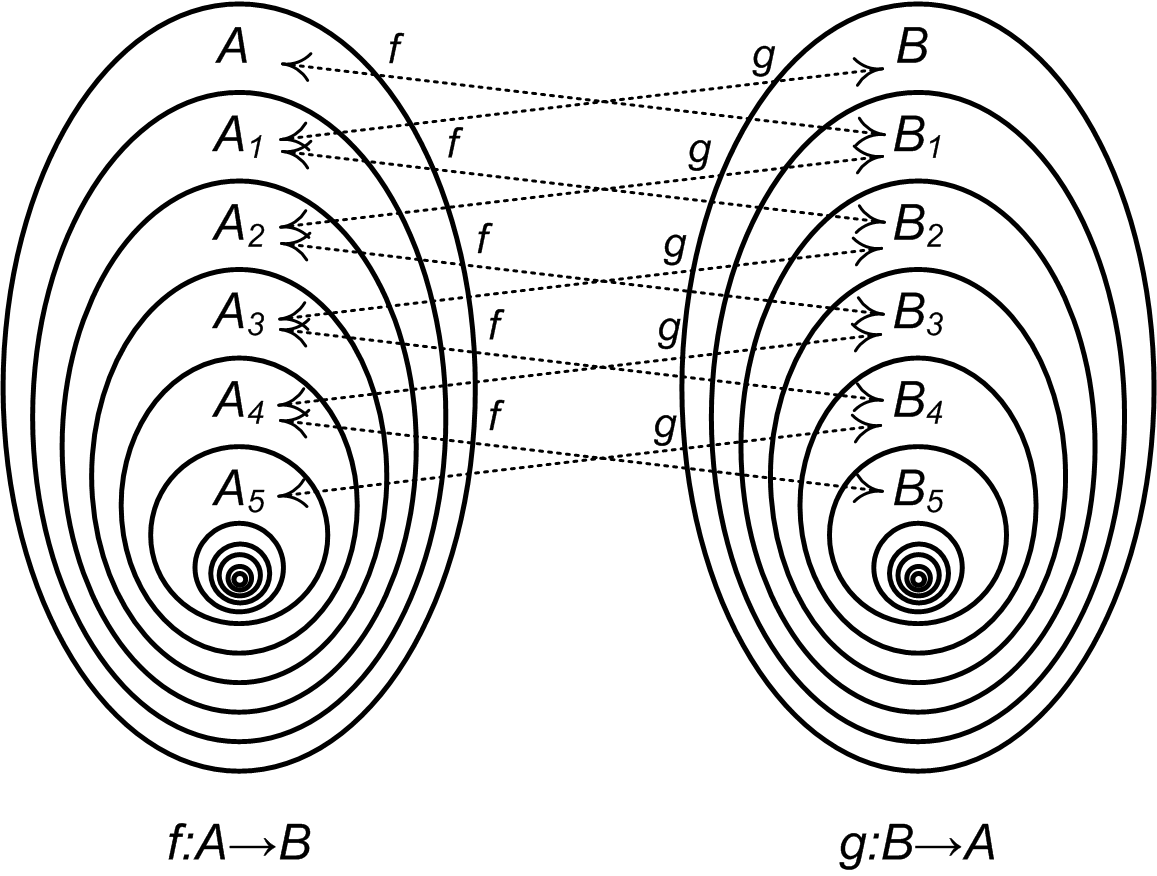
\includegraphics{fig/kantorBernstein1}
    \caption{$A\leq B$ и $B\leq A$}
    \label{fig:kantorBernstein1}
\end{figure} 

\begin{figure}
    \centering
    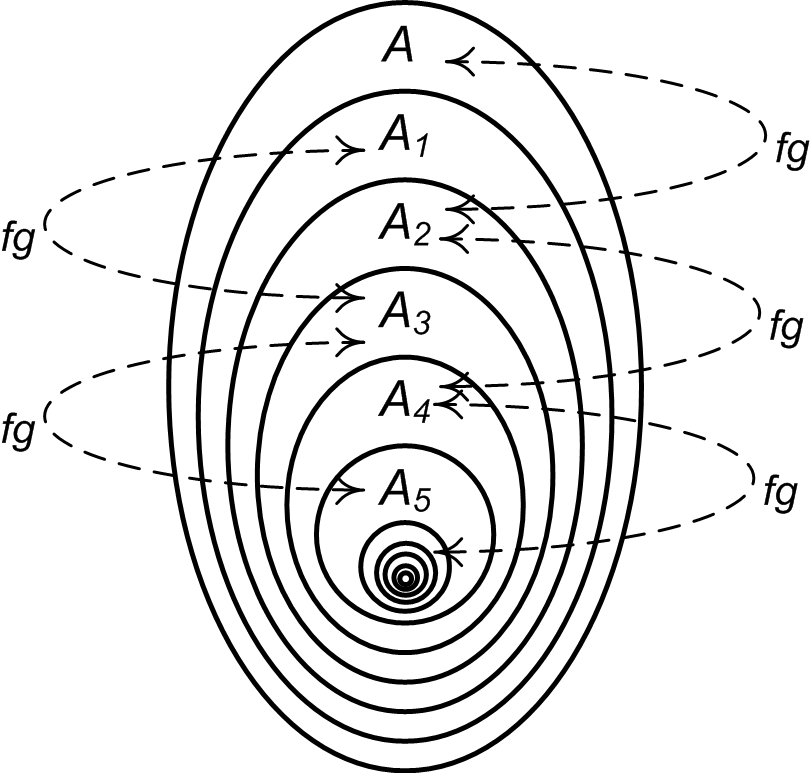
\includegraphics{fig/kantorBernstein2}
    \caption{$f\cdot g:M_{i}\leftrightarrow M_{i+2}$}
    \label{fig:kantorBernstein2}
\end{figure} 

\begin{figure}
    \centering
    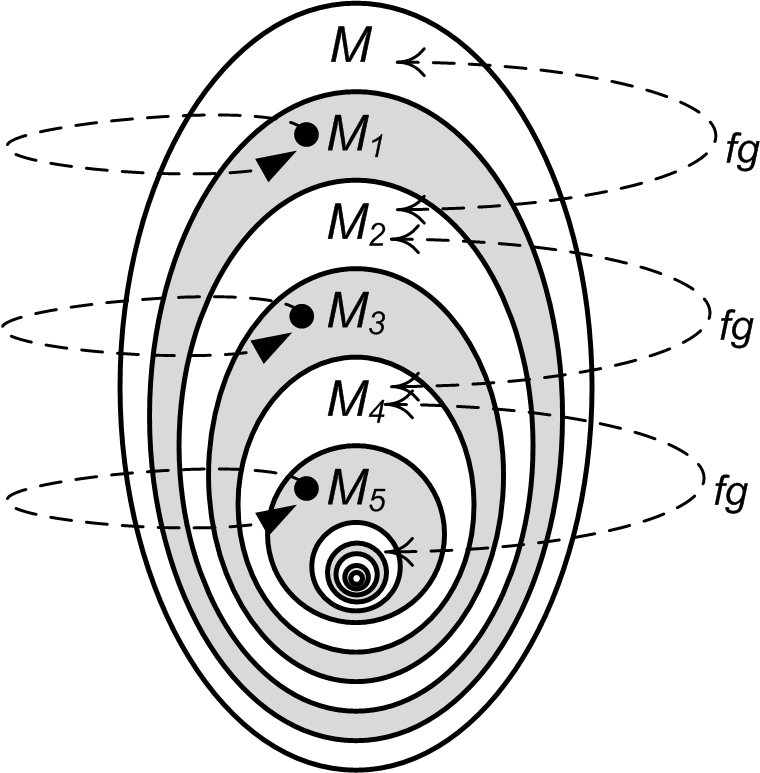
\includegraphics{fig/kantorBernstein3}
    \caption{Биекция $h:A\leftrightarrow A_1$}
    \label{fig:kantorBernstein3}
\end{figure} 

Из теоремы Кантора-Бернштейна следует, что для любых множеств $A$ и $B$ существует одна и только одна из трех возможностей:
\begin{enumerate}
    \item $|A|=|B|$;
    \item $|A|<|B|$;
    \item $|A|>|B|$.
\end{enumerate}

Мощность множества называют также \emph{кардинальным числом} или \emph{кардиналом}.  Кардинал характеризует целый \emph{класс} эквивалентных множеств. При решении практических задач часто требуется заменить некоторое множество на эквивалентное ему. При условии равенства кардиналов, это можно сделать.

Кардиналом для \emph{конечного} множества $A$ является натуральное число, равное количеству элементов множества $A$.

Для кардиналов \emph{конечных} множеств справедливо, например, что:
\begin{enumerate}
    \item Если $|A|=m$, $|B|=n$, то $|A\cup B|=m+n-|A\cap B|$;
    \item Если $|A|=m$, $|B|=n$, то $|A\times B|=m\cdot n$;
    \item Если $|A|=m$, $|B|=n$, то $|A^B|=m^n$.
\end{enumerate}

Видно, что кардиналы можно складывать, перемножать и возводить в степень.

Возведение множества в степень множества $A^B$ ранее не определялось. Множество $A^B$ состоит из всех возможных отображений множества $B$ на множество $A$:
\[
    A^B=\{f|f:B\to A\}.
\]

Например, булеан множества $M$, обозначается как $2^M$, где под <<$2$>> понимается любое двухэлементное множество, например, $\{0,1\}$. То есть <<$2$>> --- кардинал.
\begin{exampl} $M=\{a,b\}$. Булеан $2^M$ и множество $\{0,1\}^M$, эквивалентны:
    \[
    \begin{array}{c|c}
        2^M = \{          & \{0,1\}^M=\{                \\ \hline
        \{\emptyset\},    & \{a\mapsto 0, b\mapsto 0\}, \\
        \{a\},            & \{a\mapsto 1, b\mapsto 0\}, \\
        \{b\},            & \{a\mapsto 0, b\mapsto 1\}, \\
        \{a,b\}           & \{a\mapsto 1, b\mapsto 1\}  \\ \hline
        \}                &\}
    \end{array}
    \]
    \qed
\end{exampl}

Аналогично можно смотреть на степень множества $M^n$, где $n\in\mathbb{N}$ --- кардинал конечного множества.
\begin{exampl} $M=\{a,b\}$. $M^3$ и множество $M^{\{0,1,2\}}$, эквивалентны:
    \[
    \begin{array}{l||l}
        M^3 = \{    & M^{\{0,1,2\}}=\{              \\ \hline\hline
        \{a,a,a\},    & \{0\mapsto a, 1\mapsto a, 2\mapsto a\}, \\
        \{a,a,b\},    & \{0\mapsto a, 1\mapsto a, 2\mapsto b\}, \\
        \{a,b,a\},    & \{0\mapsto a, 1\mapsto b, 2\mapsto a\}, \\
        \{a,b,b\},    & \{0\mapsto a, 1\mapsto b, 2\mapsto b\}, \\
        \{b,a,a\},    & \{0\mapsto b, 1\mapsto a, 2\mapsto a\}, \\
        \{b,a,b\},    & \{0\mapsto b, 1\mapsto a, 2\mapsto b\}, \\
        \{b,b,a\},    & \{0\mapsto b, 1\mapsto b, 2\mapsto a\}, \\
        \{b,b,b\}     & \{0\mapsto b, 1\mapsto b, 2\mapsto b\}  \\ \hline\hline
        \}          &\}
    \end{array}
    \]
    \qed
\end{exampl}


\section{Мощность бесконечных множеств}

Для бесконечных множеств кардинал --- особое понятие. И при соответствующих операциях над бесконечными множествами такие кардиналы ведут себя по-особенному. 

Будь кардинал бесконечного множества обычным числом, то, например, можно было ожидать, что $|\mathbb{N}\times\mathbb{N}|=|\mathbb{N}^2|=\aleph_0^2$. Однако можно доказать, что $\mathbb{N}\times\mathbb{N}\sim\mathbb{N}$. То есть $|\mathbb{N}^2|=|\mathbb{N}|=\aleph_0$. 
\begin{exampl}
    $|\mathbb{N}^2|=|\mathbb{N}|=\aleph_0$.
\end{exampl}
\begin{proof}
    По определению множество $\mathbb{N}^2=\mathbb{N}\times\mathbb{N}$ задается как $\{(m,n)|m,n\in\mathbb{N}\}$. На координатной плоскости изобразим точки с натуральными координатами (см. рис. \ref{fig:diagonalKantor}). Если удастся построить биекцию $f:\mathbb{N}\leftrightarrow\mathbb{N}^2$, то тем самым докажем $|\mathbb{N}^2|=|\mathbb{N}|$. Видно:
    \[
        \begin{split}
            f:\mathbb{N}\leftrightarrow\mathbb{N}^2=\\
            \{
                0\mapsto(0,0),\\
                %
                1\mapsto(0,1),
                2\mapsto(1,0),\\
                %
                3\mapsto(0,2),
                4\mapsto(1,1),
                5\mapsto(2,0),\\
                %
                6\mapsto(0,3),
                7\mapsto(1,2),
                8\mapsto(2,1),
                9\mapsto(3,0),\\ \ldots
            \}
        \end{split}
    \]
\end{proof}

\begin{figure}
    \centering
    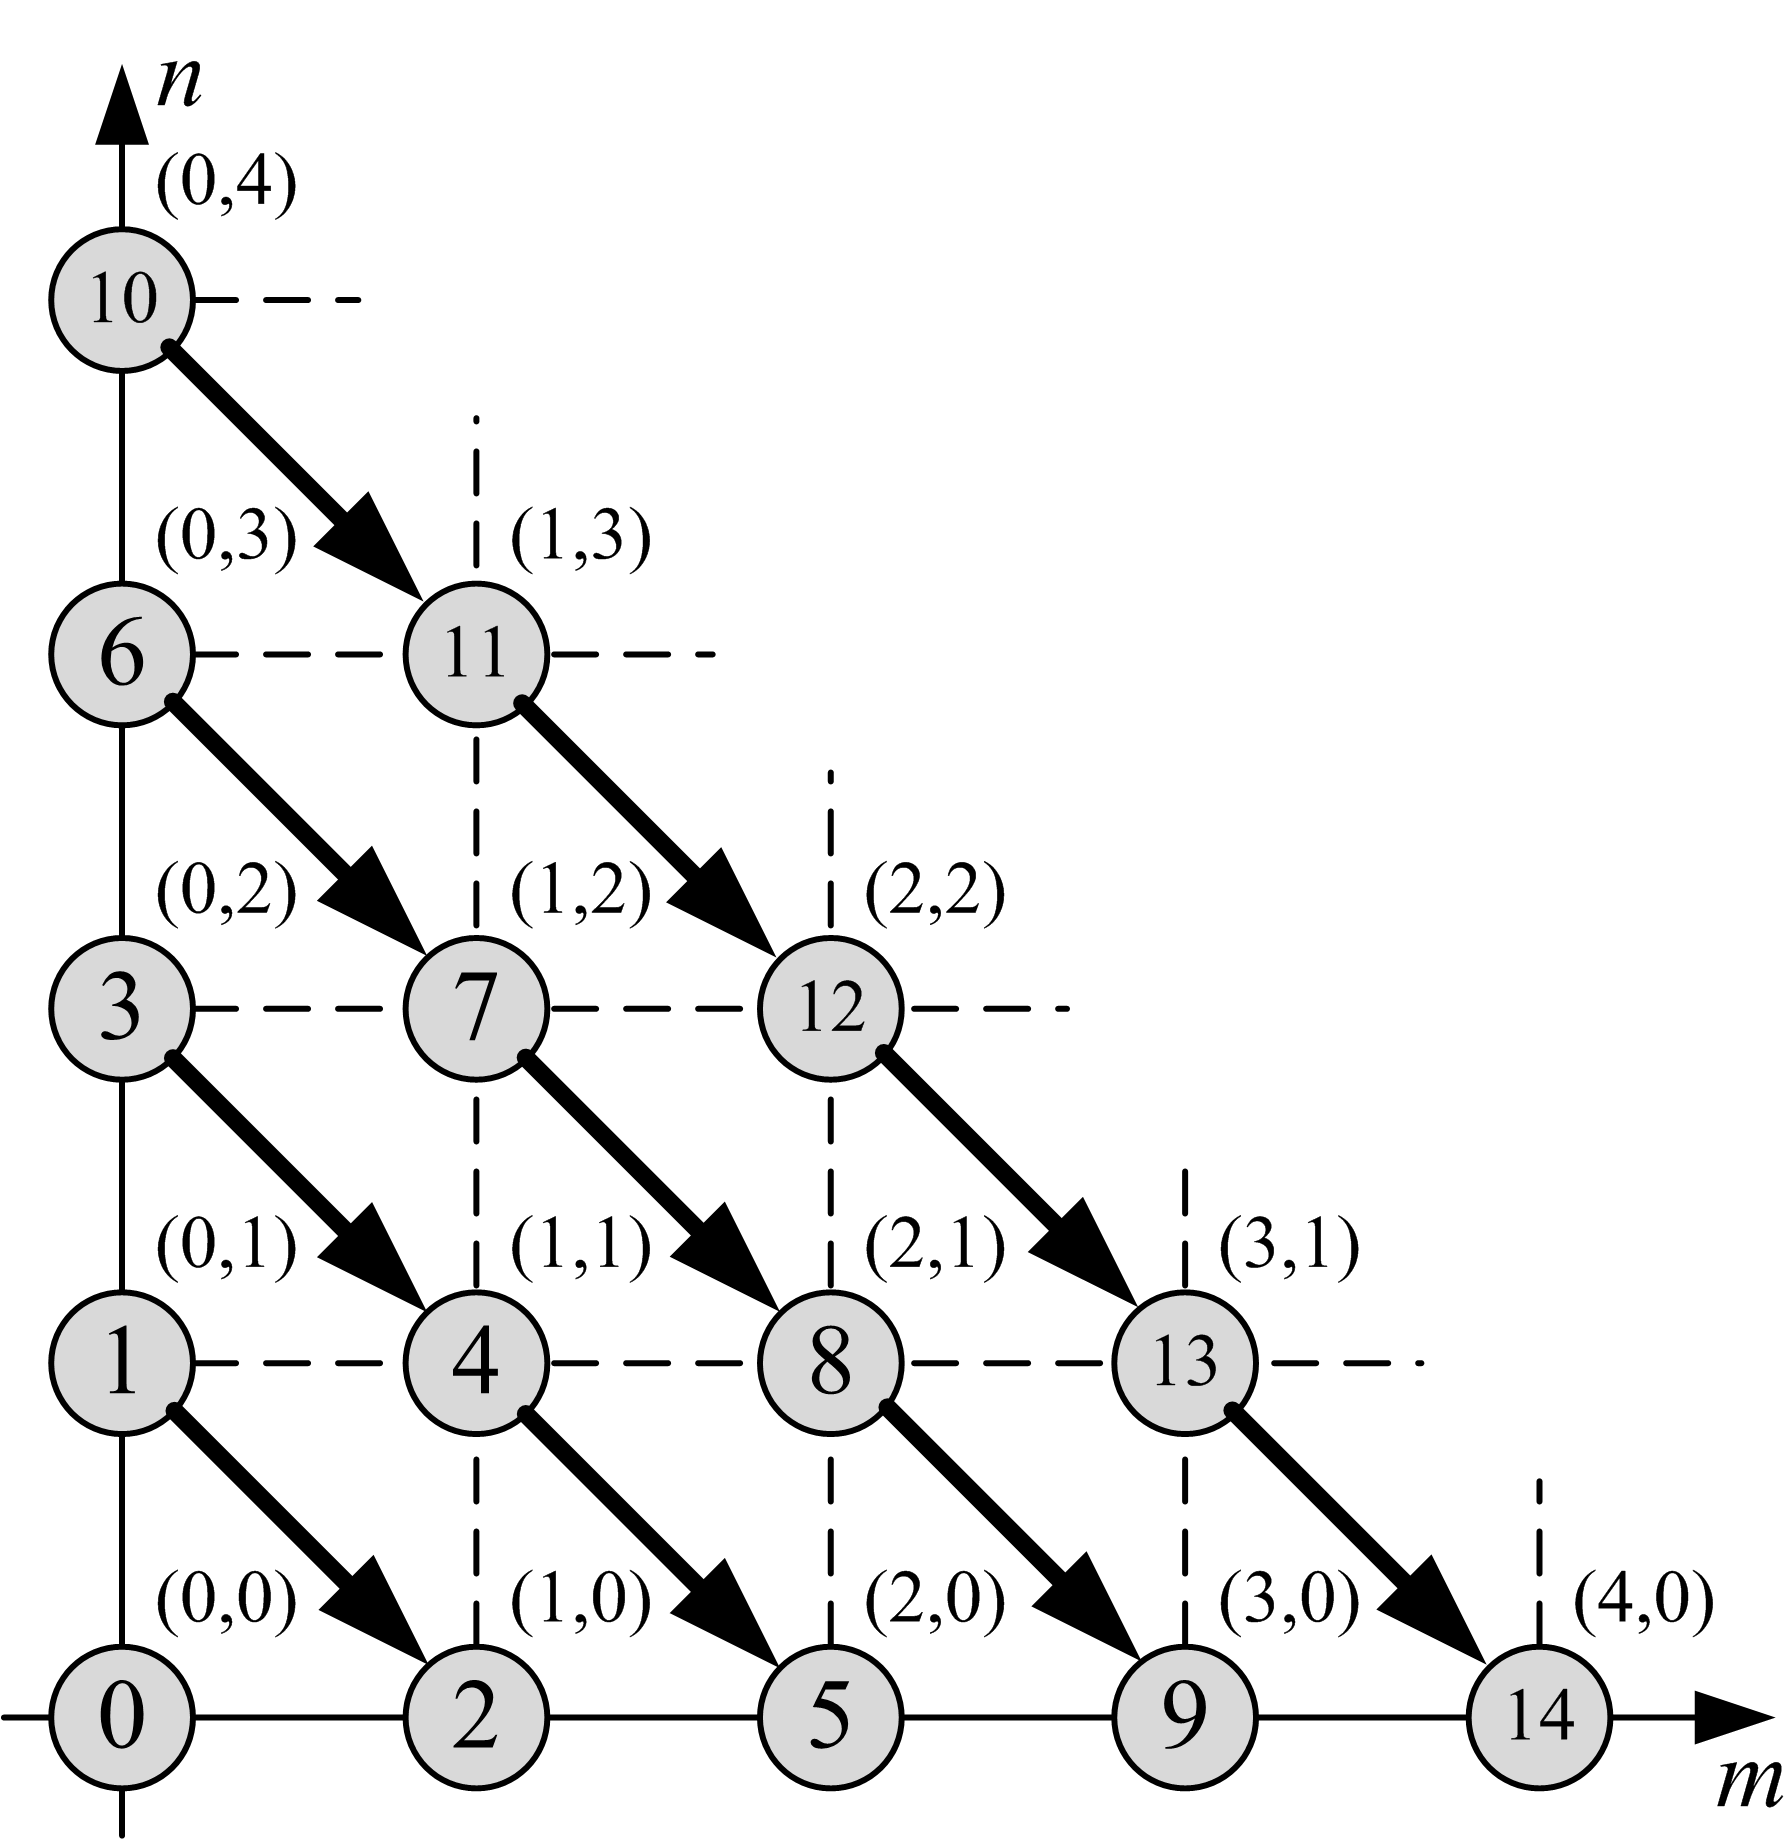
\includegraphics{fig/diagonalKantor}
    \caption{$f:\mathbb{N}\leftrightarrow\mathbb{N}^2$. Диагональная процедура Кантора}
    \label{fig:diagonalKantor}
\end{figure} 

Более того, справедливо, что:
\begin{itemize}
    \item $(\mathbb{N}\sim\mathbb{N}^n)\Leftrightarrow (|\mathbb{N}^n|=\aleph_0)$;
    \item $(\mathbb{N}\sim\bigcup_{n\in\mathbb{N}}\mathbb{N}^n) \Leftrightarrow (|\bigcup_{n\in\mathbb{N}}\mathbb{N}^n|=\aleph_0)$.
\end{itemize}

Но на $\aleph_0$ кардиналы бесконечных множеств не заканчиваются. Существуют бесконечные множества \emph{б\'{о}льших} мощностей.

\begin{Theor}[теорема Кантора]\label{ch:pwr:kantor}
    Для любого множества $M$ выполняется $|M|<2^{|M|}$.
\end{Theor}
\begin{proof}
    Так как для любого множества $M$ выполняется $|2^M|=2^{|M|}$, то необходимо показать, что $|M|\leq|2^M|$ и $|M|\neq|2^M|$. Функция $f:M\xrightarrow{\text{в}}2^M$, определенная по правилу $f(x)=\{x\}$, очевидно, инъективна, а тогда справедливо, что $|M|\leq|2^M|$. Теперь предположим, что $|M|=|2^M|$. Тогда существует биекция $\varphi:M\leftrightarrow 2^M$. Рассмотрим множество $K=\{x|x\in M,x\not\in\varphi(x)\}$. Поскольку $\varphi$ --- биекция и $K\subseteq M$, т.е. $K\in 2^M$, то существует $s\in M$, такое, что $\varphi(s)=K$. Если $s\in K$, то из определения $K$ получаем, что $s\not\in(K=\varphi(k))$. Если $s\not\in K$, то $s\not\in\varphi(s)$ и из определения $K$ следует, что должно выполняться $s\in K$. Противоречие показывает, что биекция $\varphi$ существовать не может.
\end{proof}

Для бесконечных множеств кардиналы имеют вид: $\aleph_0$, $2^{\aleph_0}$, $2^{2^{\aleph_0}}$,\ldots

\begin{exampl}
    $2^\mathbb{N}\sim 10^\mathbb{N}\sim \mathbb{N}^\mathbb{N}$.
\end{exampl}
\begin{proof}
    Поскольку неравенства $2^\mathbb{N}\leq 10^\mathbb{N}\leq \mathbb{N}^\mathbb{N}$ очевидны, то по теореме Кантора-Бернштейна (см. теорему \ref{Theor:KantorBernstain}) достаточно показать, что существует $\varphi:\mathbb{N}^\mathbb{N}\xrightarrow{\text{в}}2^\mathbb{N}$. Это фактически означает $\varphi$ кодирует все возможные последовательности натуральных чисел с помощью последовательностей из нулей и единиц. Для последовательности $f\in\mathbb{N}^\mathbb{N}$ 
    \[f=f_0f_1\cdots f_n\cdots\]
    определим последовательность $\varphi(f)\in 2^\mathbb{N}$ так:
    \[
        \underbrace{1,1,\ldots,1}_{f_0},0,
        \underbrace{1,1,\ldots,1}_{f_1},0,\ldots,0,
        \underbrace{1,1,\ldots,1}_{f_n},0,\ldots
    \]
    
    Определенная таким образом $\varphi$, очевидно является  биекцией. Например, если
    \[\varphi(f)=0,1,1,1,0,0,1,1,1,1,1,0\cdots\], то легко определяется \[f=0,3,0,5,\ldots\]
\end{proof}

Если $A\sim 2^{\mathbb{N}}$, то множество $A$ называется \emph{континуальным} или \emph{континуумом}: $|A|=2^{\aleph_0}$. Слово \emph{континуум} означает \emph{непрерывный}. Далее показано, например, что <<непрерывное>> множество вещественных чисел $\mathbb{R}$ эквивалентно всем возможным подмножествам множества натуральных чисел $2^\mathbb{N}$ и имеет мощность $|\mathbb{R}|=2^{\aleph_0}$.

\begin{exampl}
    $\mathbb{R}\sim [0,1]$
\end{exampl}
\begin{proof}
    Доказать, что мощности отрезка $[0,1]$ и интервала $(0,1)$ равны, можно задав биекцию:
    \[
        \varphi(x)=
        \begin{cases}
            x,&\text{если $x\neq 0,x\neq\frac{1}{n},n\in\mathbb{N},n>0)$},\\
            \frac{1}{2},&\text{если $x=0$},\\
            \frac{1}{3},&\text{если $x=1$},\\
            \frac{1}{n+2},&\text{если $x=\frac{1}{n},n\in\mathbb{N},n>1$}.\\
        \end{cases}
    \]
    В свою очередь биекция (см. рис. \ref{fig:tanIsContToR}) $\psi(x)=\tan(\pi(x-\frac{1}{2}))$ определяет эквивалентность интервала $(0,1)$ и множества $\mathbb{R}$. Тогда биекция $\psi(\varphi(x))$ определяет $[0,1]\sim\mathbb{R}$
\end{proof}

\begin{figure}
    \centering
    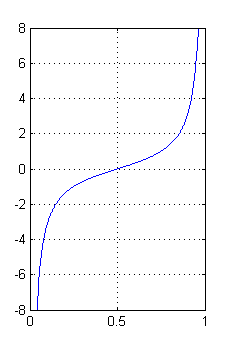
\includegraphics{fig/tanx}
    \caption{Биекция $\psi(x)=\tan(\pi(x-\frac{1}{2}))$}
    \label{fig:tanIsContToR}
\end{figure} 

Отрезок вещественной оси $[0,1]$ также называется континуумом.

\begin{Theor}
    $|\mathbb{R}|=2^{\aleph_0}$
\end{Theor}
\begin{proof}
    Любое вещественное число $X$ из $[0,1]$ можно задать в десятичном представлении бесконечной последовательностью:
    \[
        X\mapsto(0.a_1a_2\cdots a_n\cdots)_{10},
    \]
    где $n\in\mathbb{N}$ и $a_i\in\{0,\ldots,9\}$. При этом число определяется как
    \[
        X=\sum_{i\geq 1,i\in\mathbb{N}}a_i\cdot \frac{1}{10^i}.
    \]
    
    Видно, что $[0,1]\sim 10^\mathbb{N}$. Исходя из ранее доказанного:$10^\mathbb{N}\sim 2^\mathbb{N}$ и $\mathbb{R}\sim[0,1]$, заключаем $|\mathbb{R}|=2^{\aleph_0}$.
\end{proof}

Счетные и континуальные множества наиболее употребимы на практике. Но кардиналов бесконечных множеств (согласно теореме Кантора см. теорему \ref{ch:pwr:kantor}) бесконечно много, например $|2^\mathbb{R}|=2^{2^{\aleph_0}}$ --- множество всех подмножеств вещественных чисел мощнее континуума.


\section*{Задания}
\addcontentsline{toc}{section}{Задания}

\begin{enumerate}
    \item В группе из $40$ студентов все вычислители или отличники, и других нет. Вычислителей $30$, отличников $35$. Сколько вычислителей --- отличники?

    \item На острове $1000$ человек. Из них детей $400$, а взрослых женщин $350$. Сколько на острове 
    \begin{enumerate}
        \item женщин и детей?
        \item взрослых?
        \item взрослых мужчин?
    \end{enumerate}

    \item Сколько натуральных чисел в диапазоне $[1,200]$ делятся (+ не делятся) на:
    \begin{enumerate}
        \item $2$ или $3$;
        \item $6$ или $21$;
        \item $2$ или $3$ или $7$;
        \item $3$ или $10$ или $14$.
    \end{enumerate}
    
    \item Сколько натуральных чисел в диапазоне $[100,500]$ делятся (+ не делятся) на:
    \begin{enumerate}
        \item $3$ или $5$;
        \item $8$ или $12$;
        \item $4$ или $6$ или $15$;
        \item $6$ или $10$ или $15$.
    \end{enumerate}
    
    \item Доказать, что $|\mathbb{N}^3|=\aleph_0$.
    
    \item Каким числам соответствуют русские слова:
    \begin{enumerate}
        \item <<Я>>
        \item <<МАМА>>
        \item <<ПАПА>>
        \item <<ДОМ>>
        \item <<РОД>>
        \item <<ВЫСОКОПРЕВОСХОДИТЕЛЬСТВО>>\footnote{Дайте хотя бы оценку количества цифр в десятичном представлении этого числа}
    \end{enumerate}
    если 
    \[f:\text{Азбука}\to\mathbb{N} = 
        \text{
            \begin{tabular}{c|cccccccccc}
                f&0&1&2&3&4&5&6&7&8&9\\
                \hline
                 &А&Б&В&Г&Д&Е&Ё&Ж&З&И\\
                1&Й&К&Л&М&Н&О&П&Р&С&Т\\
                2&У&Ф&Х&Ц&Ч&Ш&Щ&Ъ&Ы&Ь\\
                3&Э&Ю&Я& & & & & & & 
            \end{tabular}
        }
    \]
    где <<$\text{Азбука}$>> --- русский алфавит.
    
    %множество всех слов конечного алфавита счетно $\aleph_0$
    %множество всех предложений из слов континуально ${\aleph_0}^{\aleph_0}$!
    %${\aleph_0}^{\aleph_0}=2^{\aleph_0}$.
    %$M\sim\mathbb{R}\sim[0,1]$
    \item Какова мощность множества $M$ всех возможных предложений из слов русского алфавита $T$?
    
    \item Множество всех пар из $\mathbb{N}^2$, оказывается счетно! Приведите функцию $f:\mathbb{N}^2\leftrightarrow\mathbb{N}$. Найдите $f(100,100)$. Найдите пару $(x,y)=f^{-1}(2048)$.

    
    \item Докажите, что множество рациональных чисел $\mathbb{Q}$ --- счетно.
    
    \item Приведите пример регулярного выражения, порождающего множество $M$, такое, что:
    \begin{enumerate}
        \item $|M|=7$;
        \item $|M|=\aleph_0$;
        \item $|M|=2^{\aleph_0}$.
    \end{enumerate}
    
    \item Приведите пример регулярных выражений, определяющих бесконечные регулярные множества $A$ и $B$, такие, что $A\subset B$ и $|A|=|B|$.
    
    \item Докажите, что диапазоны чисел $x\in\mathbb{R}$ эквивалентны:
    \begin{enumerate}
        \item $[0,1)\sim(0,1)$;
        \item $(0,1]\sim(0,1)$;
        \item $[0,1]\sim(0,1)$;
        \item $[m,n]\sim(0,1)$, $m,n\in\mathbb{N}$.        
    \end{enumerate}
    
\end{enumerate}
